\chapter{LoongArch2K1000适配}

在NPUcore中,我们在os/arc/arch里对所有涉及硬件交互的组件均更新为LoongArch架构版本。
如代码片段\ref{code:content2}所示,我们的硬件设备约束,都放入arch中的la64文件夹,其中分为board,register,trap三个子文件夹。
在board中,2k1000.rs用于规定与2K1000开发板相关的串口宏(这个串口地址也是我们自己摸出来的,未找到任何官方说明)。
在register中,我们封装了base(基本寄存器),mmu(tlb相关),ras,timer的所有硬件相关寄存器。
在trap中,我们主要规定了内核态陷入方面所必须的类型与限制。
由于有关内存模块的适配最为艰难,因此,我们后面重点讲述这部分内容,同时也会提到基于2K1000-QEMU的适配。

\begin{lstlisting}[language={bash}, label={code:content2},
	caption={“os/arc/arch”目录树}]
    |-- la64
    |   |-- board
    |   |   |-- 2k1000.rs
    |   |-- config.rs
    |   |-- entry.asm
    |   |-- kern_stack.rs
    |   |-- la_libc_import.rs
    |   |-- laflex.rs
    |   |-- mod.rs
    |   |-- register
    |   |   |-- base
    |   |   |   |-- acpi.rs
    |   |   |   |-- badi.rs
    |   |   |   |-- badv.rs
    |   |   |   |-- crmd.rs
    |   |   |   |-- ecfg.rs
    |   |   |   |-- eentry.rs
    |   |   |   |-- era.rs
    |   |   |   |-- estat.rs
    |   |   |   |-- euen.rs
    |   |   |   |-- misc.rs
    |   |   |   |-- mod.rs
    |   |   |   |-- prcfg.rs
    |   |   |   |-- prmd.rs
    |   |   |   |-- rvacfg.rs
    |   |   |-- macros.rs
    |   |   |-- mmu
    |   |   |   |-- asid.rs
    |   |   |   |-- dmw.rs
    |   |   |   |-- mod.rs
    |   |   |   |-- pgd.rs
    |   |   |   |-- pwch.rs
    |   |   |   |-- pwcl.rs
    |   |   |   |-- stlbps.rs
    |   |   |   |-- tlbehi.rs
    |   |   |   |-- tlbelo.rs
    |   |   |   |-- tlbidx.rs
    |   |   |   |-- tlbrbadv.rs
    |   |   |   |-- tlbrehi.rs
    |   |   |   |-- tlbrelo.rs
    |   |   |   |-- tlbrentry.rs
    |   |   |   |-- tlbrera.rs
    |   |   |   |-- tlbrprmd.rs
    |   |   |-- mod.rs
    |   |   |-- ras
    |   |   |   |-- merrctl.rs
    |   |   |   |-- merrentry.rs
    |   |   |   |-- merrera.rs
    |   |   |   |-- mod.rs
    |   |   |-- timer
    |   |       |-- mod.rs
    |   |       |-- tcfg.rs
    |   |       |-- ticlr.rs
    |   |-- sbi.rs
    |   |-- switch.S
    |   |-- switch.rs
    |   |-- syscall_id.rs
    |   |-- time.rs
    |   |-- tlb.rs
    |   |-- trap
    |       |-- context.rs
    |       |-- mem_access.rs
    |       |-- mod.rs
    |       |-- trap.S
    |-- mod.rs
    
\end{lstlisting}

\section{LoongArch内存模块适配}

\subsection{内存地址映射布局}
LoongArch 的虚拟映射模式内存机理如下图:
\begin{figure}[htp]
    \centering
    \label{fig:mmu}
    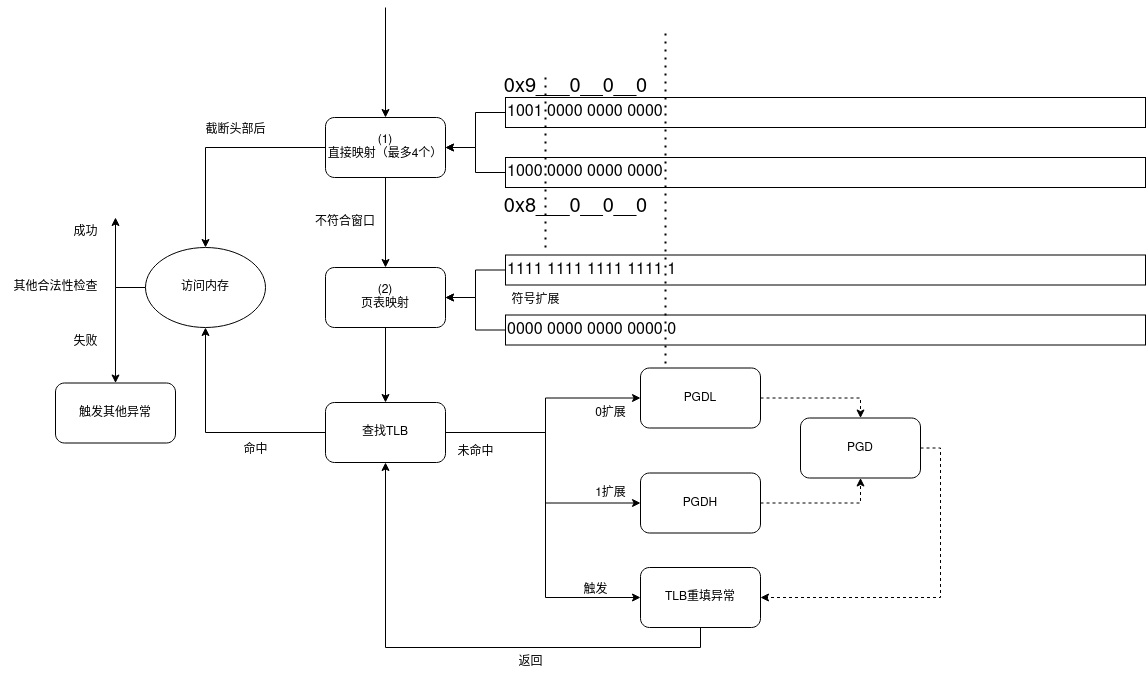
\includegraphics[width=0.8\linewidth]{figs/LA虚拟内存映射.png}
    \caption{LoongArch的虚拟映射模式}
\end{figure}
\begin{enumerate}
    \item 首先,检查是否符合直接映射窗口(通过DMW0~3四个CSR进行映射),
    如果其高4位相同则认为是符合,则将其他位数截断,作为物理地址访问。
    \item 其次,如果不是,则检查是否符号扩展,是则尝试查找 TLB,否则出发
    异常,在miss后,如果是1扩展则PGD为PGDH,0 扩展为 PGDL,
    然后触发TLB重填异常,ertn 返回后重新进行TLB查找。如果此时
    没有对应的TLB,则触发页无效异常。
    \item 此外, 对 DMW 的权限是: 0号和1号窗口是RWX, 2号和3号窗口是
    RW(不可执行)。 每个窗口可以单独设置自己的缓存一致性类型。

\end{enumerate}

由于 LoongArch 的特殊特性,NPUcore-IMPACT内存布局采取了和RISC-V下不同的方案:
\begin{enumerate}
    \item 对用户态,使用0扩展地址作为虚拟空间;
    \item 对内核态,用0扩展地址空间访问物理内存,然后对页表映射使用1扩展的地址。
\end{enumerate}
这样做可以用直接继承原版NPUcore的部分内存布局,无需为了利用 LA 的
直接映射窗口就大量修改代码,在物理地址上按位或大量的0x9000000090000000,减少代码出错空间。而且,这样可以利用直接映射减小恒等映射的开销,在上下文无需存储页表地址,可以直接切换地址空间。

\subsubsection{跳转}
从u-boot获得控制权时,引导程序提供了几个已经映射好的段: 0x9000
段 (一致可缓存), 和0x8000段 (无缓存直接访问内存), 前者使用 DMW1,
后者 DMW0(可能随u-boot版本不同而不同)。

由于地址空间中0段地址是不被映射的,因此需要某些方法先设置
DMW映射0段,再让PC跳转到该地址(NPUcore内核态的PC是在物
理地址上的)。为此, 我们的启动代码la64/entry.asm需要进行如下设计(如代码片段\autoref{code:entry})。

\begin{lstlisting}[language={riscv}, label={code:entry},
	caption={la64/entry.asm}]
_start:
    pcaddi      $t0,    0x0
    srli.d      $t0,    $t0,    0x30
    slli.d      $t0,    $t0,    0x30    # 位移删去物理地址
    addi.d      $t0,    $t0,    0x11    # 计算当前的窗口CSR值
    csrwr       $t0,    0x181           # 上面代码保证窗口DMW0写入切换后不会被覆盖,所以先将DMW1设为当前段
    sub.d       $t0,    $t0,    $t0
    addi.d      $t0,    $t0,    0x11    # 计算0段DMW的值
    csrwr       $t0,    0x180           # 设置0段DMW的值
    pcaddi      $t0,    0x0
    slli.d      $t0,    $t0,    0x10
    srli.d      $t0,    $t0,    0x10
    jirl        $t0,    $t0,    0x10    # 跳0段的下一条指令
    # The barrier
    sub.d       $t0,    $t0,    $t0
    csrwr       $t0,    0x181           # 写入DMW1, 清零DMW1
    sub.d       $t0,    $t0,    $t0     # 加载boot_stack_top
    la.global $sp, boot_stack_top       # 跳转到rust_main
    bl          rust_main
\end{lstlisting}
注意这里没有使用\$t0=\$zero是因为在QEMU虚拟机下, 某些时候似
乎\$zero寄存器会被赋值为0(GDB提示), 因此使用手工计算的 \$t0=0。
这里先设置映射窗口, 而不是计算完0段的DMW控制寄存器数值后直接
覆盖到DMW0的原因是:如果当前PC的地址处在DMW0而非DMW1的区段内, 覆盖DMW0后PC的地址就会成为非法地址。
跳转必然发生在映射了新的区段号后,因此要先将当前的区段保存到DMW1, 然后再进行对DMW0的配置,
从而确保至少有一个DMW是PC当前的地址。

\subsection{不对齐读写问题}
当前开源的LLVM的LoongArch后端不支持生成严格对齐
的代码, 因此也导致依赖LLVM后端进行代码生成的Rustc无法编译出可
以在开发板上正常运行的代码, 这也就要求我们对NPUcore的不对齐异常手动处理。

虽然 QEMU 支持不对齐读写, 但是开发板是无法支持不对齐读写的.
如果要在 QEMU 上支持不对齐读写的检测和不对齐读写的报错, 需要开启
环境变量 DEBUG_UNALIGN=1, 否则会忽略所有的不对齐读写异常。
具体的启动命令是:DEBUG_UNALIGN=1 DEBUG_GMAC_PHYAD=0 DEBUG_MYNAND=cs=0,id=0x2cda DEBUG_MYSPIFLASH=gd25q128 \$QEMU。

如果将来LoongArch的LLVM完成了严格对齐读写的修复, 则应当可
以用target-feature开启编译器的选项:
\begin{lstlisting}[language={rust}, label={code:entry},
	caption={la64/entry.asm}]
[target.loongarch64-unknown-linux-gnu]
rustflags = ["-Ctarget-feature=-unaligned-access",
"-Clink-arg=-Tsrc/linker.ld", "-Clink-arg=-nostdlib", "-Clink-arg=-static"]
\end{lstlisting}
这个问题在C语言的GCC下是不存在的, 因此, 理论上在Rust编写
的操作系统上, 当前会由于不对齐读写存在性能瓶颈。 为了解决这个问题, 我
们需要在内核态手动模拟不对齐读写指令的执行。

内核态的不对齐异常只出现在栈上, 因为静态数据和堆上的数据结构是对齐的, 而NPUcore-LA的内核堆则是从栈上分配
的, 只有在ELF加载阶段有部分只读临时的内核页表映射。 因此, 只需要保
存内容后, 对进行逐字节解读取即可。具体来说, 为了节省内容恢复的空间, 我们直接对kernel trap的设计为:
\begin{enumerate}
    \item 内容保存不需要单独建立一个位置, 直接将寄存器上下文保存在栈上,
    因为内核的不对齐读写异常是发生在执行时, 所以直接视为一个单独
    的函数调用即可。
    \item 指令解码使用。
\end{enumerate}

内容保存的代码如下:
\begin{lstlisting}[language={riscv}, label={code:trap},
	caption={la64/trap/trap.S}]
    __kern_trap:
    # Keep the original $sp in SAVE
    csrwr $sp, CSR_SAVE    
    csrrd $sp, CSR_SAVE
    # Now move the $sp lower to push the registers
    addi.d $sp, $sp, -256
    # Align the $sp
    srli.d  $sp, $sp, 3
    slli.d  $sp, $sp, 3
    # now sp->*GeneralRegisters in kern space, CSR_SAVE->(the previous $sp)

    SAVE_GP 1 # Save $ra
    SAVE_GP 2 # Save $tp

    # skip r3(sp)
    .set n, 4
    .rept 28
        SAVE_GP %n
        .set n, n+1
    .endr
    .set n, 0
    csrrd $t0, CSR_ERA
    st.d $t0, $sp, 0

    move $a0, $sp
    csrrd $sp, CSR_SAVE
    st.d $sp, $a0, 3*8
    move $sp, $a0

    bl trap_from_kernel

    ld.d  $ra, $sp, 0
    csrwr $ra, CSR_ERA
    LOAD_GP 1
    LOAD_GP 2

    # skip r3(sp)
    .set n, 4
    .rept 28
        LOAD_GP %n
        .set n, n+1
    .endr
    .set n, 0
    
    csrrd $sp, CSR_SAVE
    ertn
\end{lstlisting}


读写的关键代码如下:
\begin{lstlisting}[language={rust}, label={code:trap},
	caption={la64/trap/trap.S}]
if op.is_store() {
                    let mut rd = gr[ins.get_rd_num()];
                    for i in 0..sz {
                        unsafe { ((addr + i) as *mut u8).write_unaligned(rd as u8) };
                        rd >>= 8;
                    }
                } else {
                    let mut rd = 0;
                    for i in (0..sz).rev() {
                        rd <<= 8;
                        let read_byte =
                            (unsafe { ((addr + i) as *mut u8).read_unaligned() } as usize);
                        rd |= read_byte;
                        //debug!("{:#x}, {:#x}", rd, read_byte);
                    }
                    if !op.is_unsigned_ld() {
                        match sz {
                            2 => rd = (rd as u16) as i16 as isize as usize,
                            4 => rd = (rd as u32) as i32 as isize as usize,
                            8 => rd = rd,
                            _ => unreachable!(),
                        }
                    }
                    gr[ins.get_rd_num()] = rd;
                }
                gr.pc += 4;
\end{lstlisting}

注意这里的rev是必须的, 因为LoongArch是小端机器, 所以高字节的先读才能被或到低位。
理论上, 还存在更快的办法, 就是判断是否跨整$2^{n}$字节, 如果不跨
过, 则用汇编选择对应字节的内容, 否则就读入两寄存器(128bits)再取各自
需要的部分组合成一个寄存器的值. 但由于其实现较为复杂, 所以我们考虑在决赛时采用。

\subsection{TLB refill与页表结构}
\subsubsection{TLB重填异常}
\begin{figure}
    \centering
    \label{fig:TLB}
    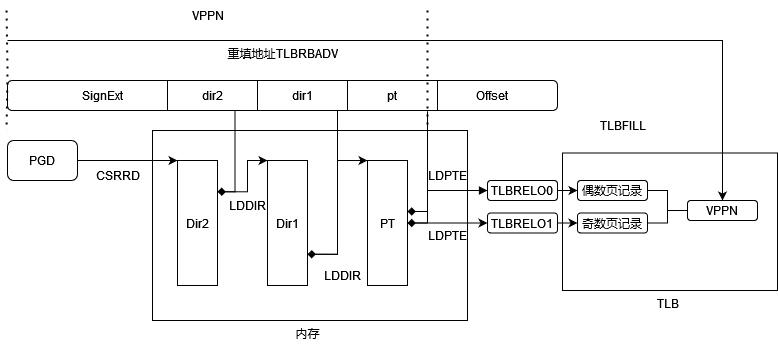
\includegraphics[width=1\linewidth]{figs/TLB重填.png}
    \caption{TLB重填}
\end{figure}
如图\autoref{fig:TLB},一旦在虚拟地址模式中被判定为页表映射的地址, 发生 TLB miss, 就会
触发 TLB 重填异常。LoongArch 目前是手动重填 TLB 的。其重填的一般
流程如下:
\begin{enumerate}
    \item 硬件提供页表地址PGD。
    \begin{enumerate}[label=$(\mathbf{\arabic*})$]
        \item  LoongArch 有两个页表 PGDL 和 PGDH,分别对应符号扩展的全1段和0段。
        \item  如果触发重填的地址来自 0 段, 则重填的页表 PGD 此时等于PGDL, 否则 PGD 此时等于 PGDH。这样一来, 页表实际上分为了高地址和低地址页表, 可以用作不同的功能。
    \end{enumerate}
    \item 硬件触发TLB异常,跳转到TLBRENTRY CSR所指向的地址。
    \item 操作系统会响应异常,通过读取PGD状态控制寄存器, 获取最高一级页表目录。
    \item 根据虚拟地址计算出对应的物理页框号。然后在主存中查找该物理页
    框的对应页表项,然后返回该页表项的物理地址. 为了加速页表重填,
    LoongArch 提供了下列特性:
    \begin{enumerate}[label=$(\mathbf{\arabic*})$]
        \item LoongArch 的 TLB 以双页形式组织,目的是减少重填次数。具
        体来说,LoongArch 的 TLB 的索引单位是 VPPN(Virtual Page
        Pair Number),为虚拟页号去掉最第一位。每个 VPPN 对应 VPN
        为 VPPN×2+VPN[12] 的一对奇数页和偶数页两页的物理地址。
        考虑到 TLB 重填的局部性,这样最多可以减少一半的 TLB 重
        填。
        \item LoongArch 提供 LDDIR 和 LDPTE 两种指令进行页表遍历,通
        过 TLBRBADV 寄存器提供重填的虚拟地址,并以此为基础获得
        各级页表的索引号。LDDIR 是用于给定非末级页表起始地址,求
        取本级页表项(或者说下一级页表起始地址),其格式为 (其中
        imm 为页表级数。以 rj 为页表起始地址,rd 为目的寄存器。):
        LDDIR rd, rj, imm。
    \end{enumerate}
    \item 返回页表项后,处理器将该对页表项用 TLBFILL 写入 TLB 中,以便
    下次使用该虚拟地址时,能够直接从 TLB 中获取物理地址信息,而不
    需要再次触发 TLB 重填。在 TLB 更新后,处理器会重新执行之前的
    指令或内存访问操作,这次操作可以直接从 TLB 中获取到物理地址。
\end{enumerate}

\subsubsection{LoongArch的页表结构}
官方手册对 LoongArch 的项目并没有清晰的叙述, 其中存在部分不明
确的地方。 具体来说(如图\autoref{fig:page}), 除了大页之外, LoongArch 并不规定页目录的页表项
格式, 所以其实际上是未定义的。
\begin{figure}
    \centering
    \label{fig:page}
    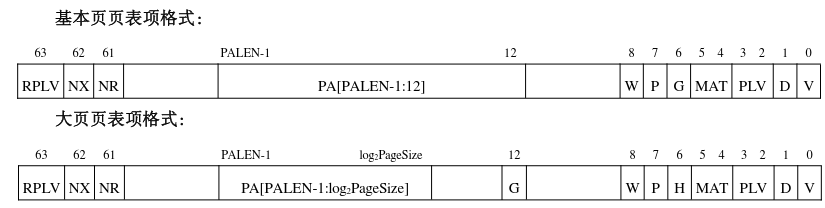
\includegraphics[width=1\linewidth]{figs/页表格式.png}
    \caption{LA页表格式}
\end{figure}
而上文提到的 LDDIR 和 LDPTE 并不检查目录项合法性, 且对非法的
页表项仍会继续寻址, 因此, 对目录项需要有手工的检测或者非法目录项的
处理方法。最简单的方法是直接模拟其他 RISC 架构的页表处理方式, 直接用汇编
代码对各层页表项进行处理。 首先, 页表是一棵前缀树, 其部分没有被映射
的节点是空的, 因此如果直接使用上述的 LDPTE 和 LDDIR, 由于其只是单
纯的将异常地址的对应段取出作相加, 因此对空的地址会计算出错误的地址,
而不是和其他 RISC 一样触发异常。 因此, 非最底层页表的叶结点 (空表项)
必须要手工判断, 并对其错误的表项, 填写无读写权限的 TLB 表项。

\begin{lstlisting}[language={riscv}, label={code:refill},
	caption={TLB refill}]
    csrwr  $t0, 0x8b
    csrrd  $t0, 0x1b
    lddir  $t0, $t0, 3
    andi   $t0, $t0, 1
    beqz   $t0, 1f

    csrrd  $t0, 0x1b
    lddir  $t0, $t0, 3
    addi.d $t0, $t0, -1
    lddir  $t0, $t0, 1
    andi   $t0, $t0, 1
    beqz   $t0, 1f
    csrrd  $t0, 0x1b
    lddir  $t0, $t0, 3
    addi.d $t0, $t0, -1
    lddir  $t0, $t0, 1
    addi.d $t0, $t0, -1

    ldpte  $t0, 0
    ldpte  $t0, 1
    csrrd  $t0, 0x8c
    csrrd  $t0, 0x8d
    csrrd  $t0, 0x0
2:
    tlbfill
    csrrd  $t0, 0x89
    srli.d $t0, $t0, 13
    slli.d $t0, $t0, 13
    csrwr  $t0, 0x11
    tlbsrch
    tlbrd
    csrrd  $t0, 0x12
    csrrd  $t0, 0x13
    csrrd  $t0, 0x8b
    ertn
1:
    csrrd  $t0, 0x8e
    ori    $t0, $t0, 0xC
    csrwr  $t0, 0x8e

    rotri.d $t0, $t0, 61
    ori    $t0, $t0, 3
    rotri.d $t0, $t0, 3

    csrwr  $t0, 0x8c
    csrrd  $t0, 0x8c
    csrwr  $t0, 0x8d
    b      2b
\end{lstlisting}

代码片段\autoref{code:refill}实现了以下功能:
\begin{enumerate}
    \item 逐层读取页表项, 如果没到最后一层, 检查读取到的页表项的合法性。合法则继续读取下一级页表项;非法则准备填入 0 页表项, 表示该页非法。
    \item 填入 0 页表项或者读取最后一层页表项结束后, 将页表大小填写为4KiB, 然后向 TLB 填入 0 地址, 表示该地址不合法。注意, 这段代码
    有 2 个需要注意的细节:
    \begin{enumerate}[label=$(\mathbf{\arabic*})$]
        \item 由于该段代码使用的 csrwr 指令在 LoongArch 下的语义是交换
        CSR 和寄存器的内容, 而非简单地将寄存器内容写入, 因此在向
        两个相同结构的 CSR 填入某个相同数值的时候, 我们需要重新读
        取之前的目的寄存器, 然后重新写入才能正确处理结果。
        \item 之所以需要对 TLB Refill exception Entry HIgh-order bits (TLBREHI)(0x8e) 的状态控制寄存器填入 0, 是因为该地址内包括页
        长度相关的域, 但该地址原本是由 ldpte 填写, 为了防止手动填写
        TLB 项导致未定义行为 (填入错误的 TLB 或虚拟机报错), 我们
        需要先对该页填写 0 地址。
    \end{enumerate}
\end{enumerate}